\newpage
\subsection*{Item Response Theory}
In this problem, you will implement an Item-Response Theory (IRT) model to predict students' correctness to diagnostic questions.

The IRT assigns each student an ability value and each question a difficulty value to formulate a probability distribution> In the one-parameter IRT model, $\beta_j$ represents the difficulty of the question j, and $\theta_i$ that represents the i-th students ability. Then, the probability that the question j is correctly answered by student i is formulated as:
\begin{equation*}
	p(c_{ij} = 1 | \theta_{i}, \beta_{j}) = \frac{exp(\theta_i - \beta_j)}{1 + exp(\theta_i -\beta_j)}
\end{equation*}
\begin{enumerate}
	\item Derive the log-likelihood $\logp(C|\theta, \beta)$ for all students and questions. Here \textbf{C} is the sparse matrix. Also, show the derivative of the log-likelihood with respect $\theta_i$ and $\beta_j$\\(Hint: recall the derivative of the logistic model with respect to the parameters.) 
\inabox{From the given equation, we know that $c_{ij}=1$ if the student answers correctly, and $c_{ij}=0$ if the student answers incorrectly.\\
	Hence, we claim the probability that
$$p(c_{ij} | \theta_i, \beta_j) = (\frac{exp(\theta_i -\beta_j)}{1 + exp(\theta_i -\beta_j)})^{c_{ij}}(\frac{1}{1 + exp(\theta_i -\beta_j)})^{(1 - c_{ij})}$$
Assume the responses from students being independently and identically distributed, thus, the joint probability is the product of the individual probabilities:
\begin{align*}
	\log_p (C| \theta, \beta) &= \sum_i \sum_j c_{ij} \log \frac{exp(\theta_i - \beta_j)}{1 + exp(\theta_i -\beta_j)} + (1 - c_{ij}) \log \frac{exp(\theta_i - \beta_j)}{1 + exp(\theta_i -\beta_j)}\\
&= \sum_i\sum_j c_{ij}(\theta_i -\beta_j) - \log (1 + exp(\theta_i -\beta_j))
\end{align*}
Then, taking the derivative of the logistic model with respect to $\theta_i, \beta_j$, we have
\begin{align*}
	\frac{\partial \log p (C | \theta, \beta)}{\partial \theta_i} &= \sum_j c_{ij} - \frac{exp(\theta_i - \beta_j)}{1 + exp(\theta_i -\beta_j)} \\
	\frac{\partial \log p (C | \theta, \beta)}{\partial \beta_j} &= - \sum_i c_{ij} + \frac{exp(\theta_i - \beta_j)}{1 + exp(\theta_i -\beta_j)}
\end{align*}}
	\item Implement missing functions that performs alternating gradient descent on $\theta$ and $\beta$ to maximize the log-likelihood. Report the hyperparameters you selected. With your chosen hyperparameters, report the training curve that shows the training and validation log-likelihoods as a function of iteration.
	\inabox{Taking hyperparameter that learning rate = 0.01, iterations = 20}
	\end{enumerate}
	\begin{center}
			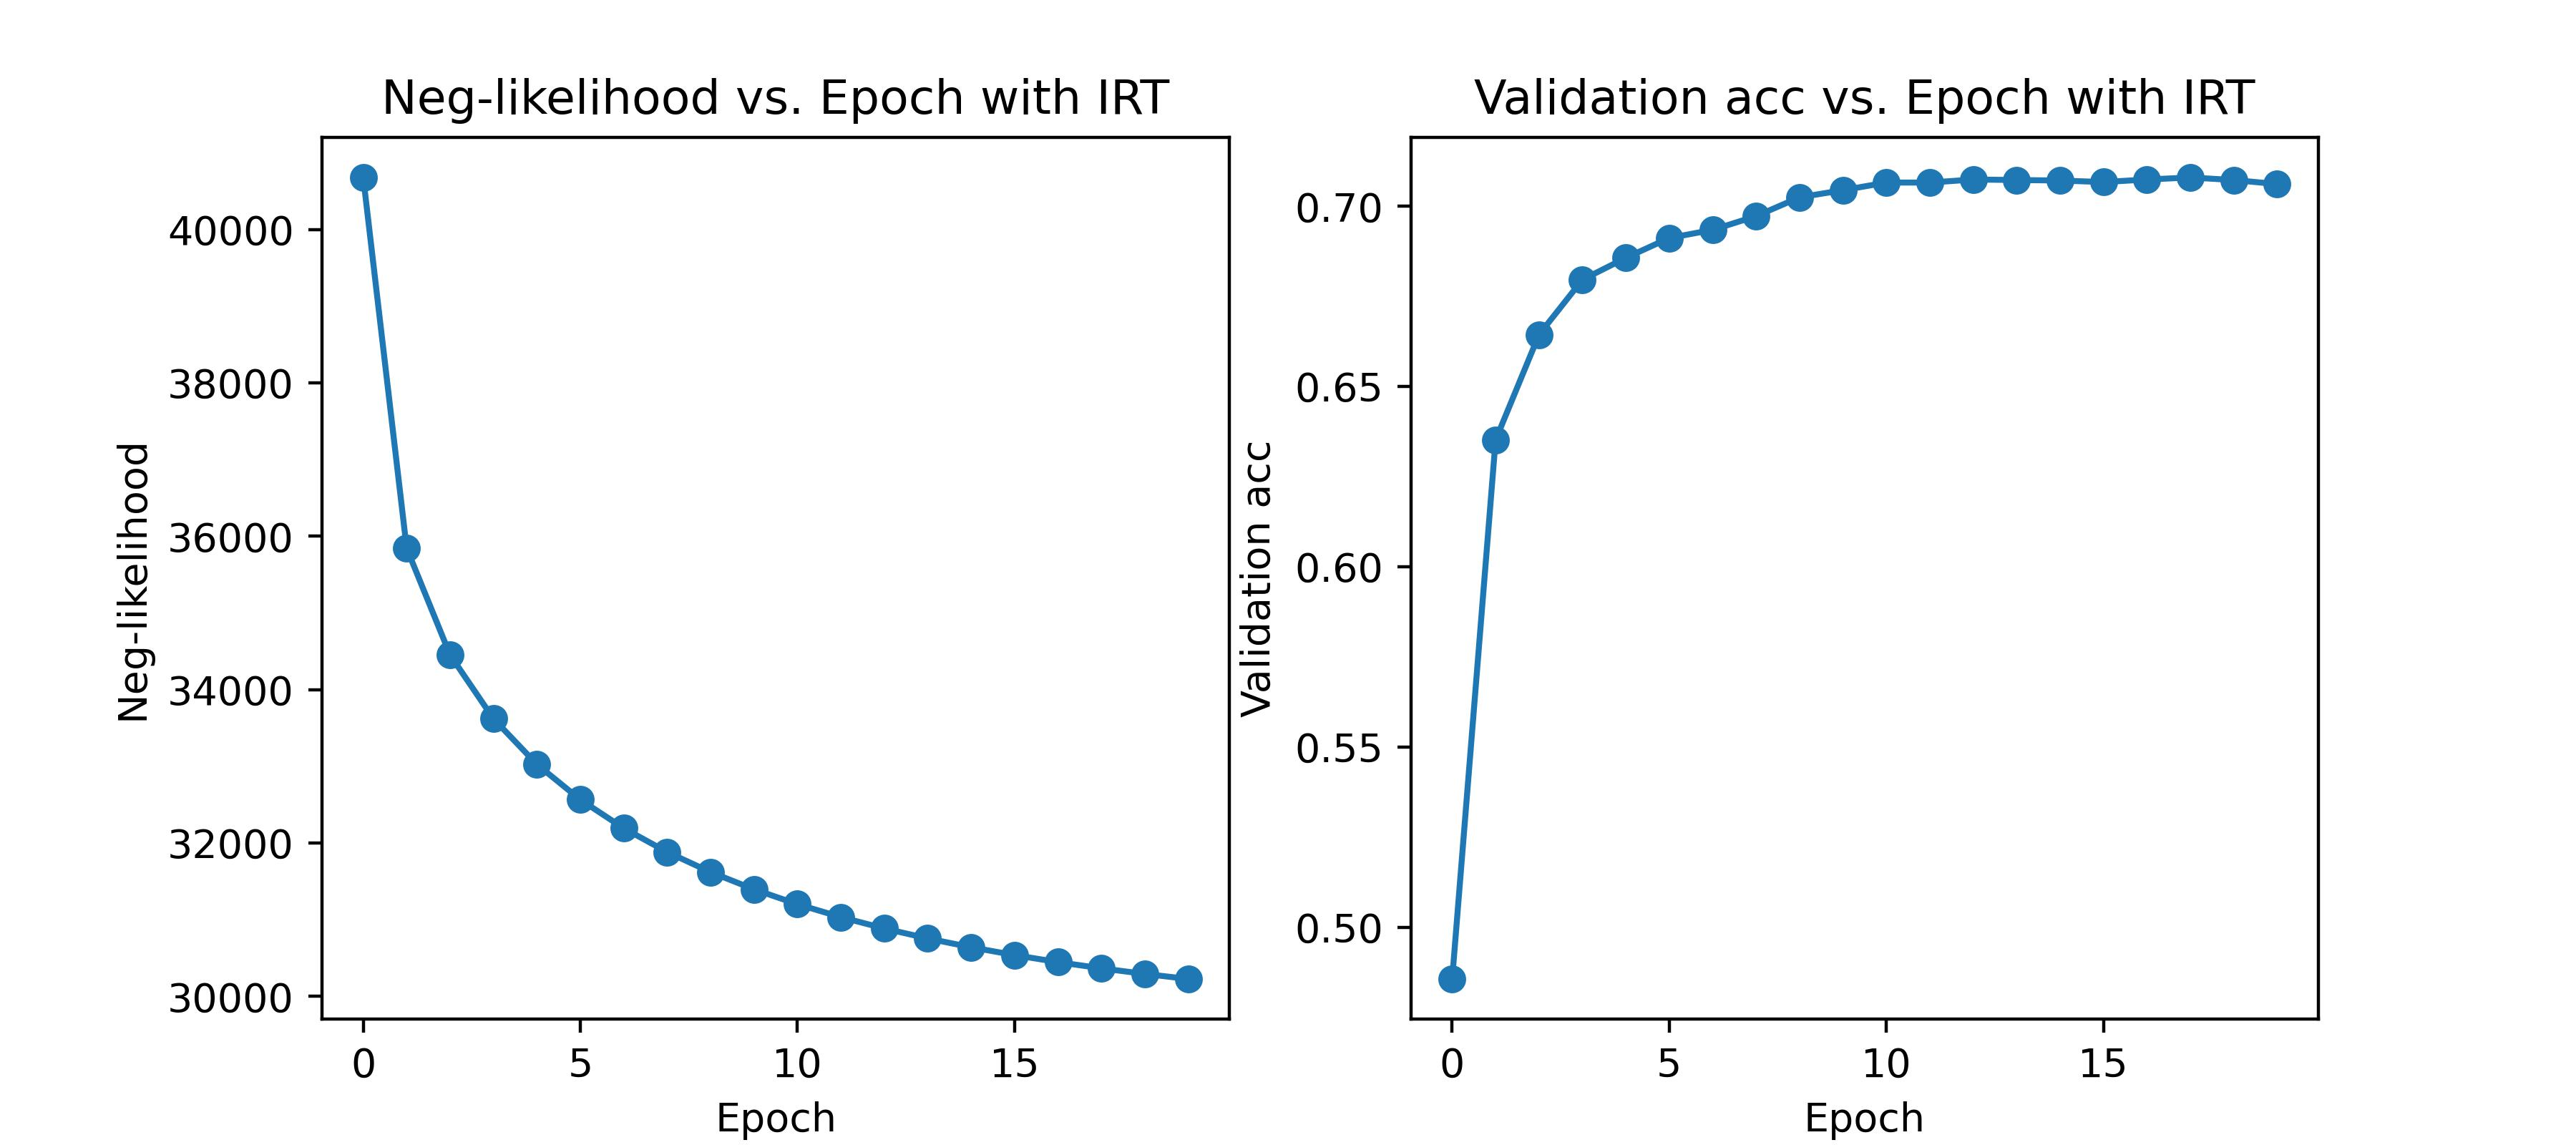
\includegraphics[scale=0.5]{../out/irt.jpg}
	\end{center}
	\begin{enumerate}
	\item [c.)] With the implemented code, report the final validation and test accuracies.
	\inabox{the final validation := 0.709991532599492\\
	final test accuracy := }
	\item [d.)]Select three questions $j_1, j_2$, and $j_3$. Using the trained $\theta$ and $\beta$, plot three curves on the same plot that shows the probability of the correct response $p(c_{ij} = 1)$ as a function of $\theta$ given a question j. Comment on the shape of the curves  and briefly describe what these curves represent.
\end{enumerate}